In this section the results of the project is summarized and the evaluation results are presented.

\subsection{Evaluation Scores}
In table \ref{tab:evaluation_performance} below the video clips chosen for the evaluation are presented, along with the achieved accuracy measurements. Training data set is a sequence of 30 minutes, where the first 5 minutes was used when training and developing the system . Evaluation data 1 is a sequence of 30 minutes. 

\begin{table}[h]
\centering
	\begin{tabular}{r | c | c | c | c | c | c }
		\emph{Sequence Name}		&  Total entered (GT) & \emph{$A_{in}$} & Total exited (GT) & \emph{$A_{out}$} & \emph{$A_{bias}$}\\
		\hline \hline
		Training data			& 108 (108) & 101 (104) & 0.99 & 0.97 & 0.99 \\
		Evaluation data 1		& 122 (141) & 0.87 & 77 (91) & 0.85 & 0.98 \\
		\end{tabular}
	\caption[System performance]{\textit{Counting performance according to the evaluation metric as described in section \ref{sec:evaluation}.}}
	\label{tab:evaluation_performance}
\end{table}

\begin{figure}[H]
\centering
\begin{subfigure}{.5\textwidth}
  \centering
  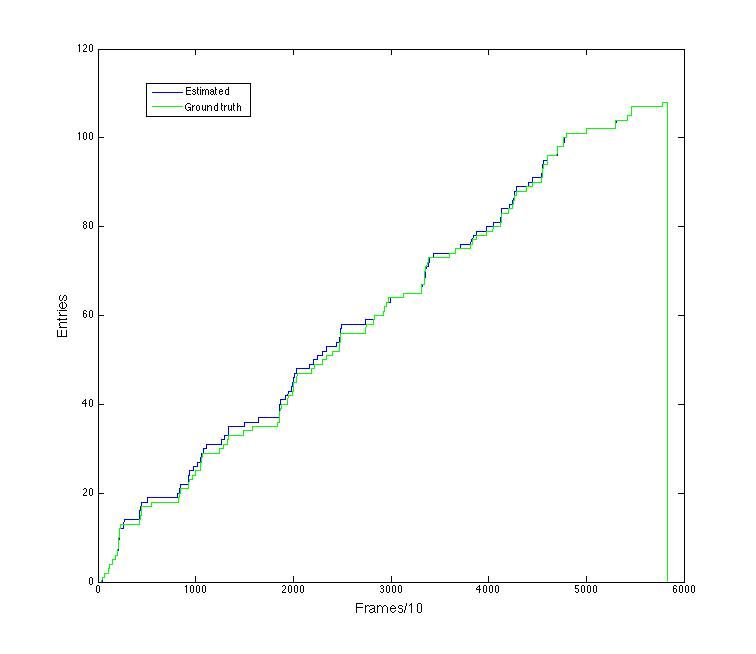
\includegraphics[width=.8\linewidth]{images/EntriesTest.png}
  \caption{Measured entries and ground truth}
  \label{fig:sub1}
\end{subfigure}%
\begin{subfigure}{.5\textwidth}
  \centering
  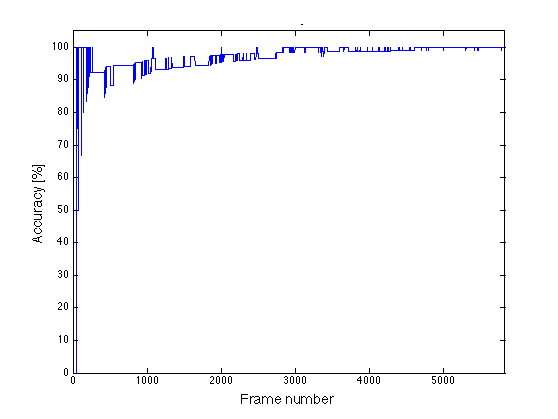
\includegraphics[width=.8\linewidth]{images/AccEntriesTest.png}
  \caption{Accuracy}
  \label{fig:sub2}
\end{subfigure}
\caption[Entries training]{\textit{Training data. Plot of measured entries, ground truth and accuracy}}
\label{fig:Entries Training data}
\end{figure}

\begin{figure}[H]
\centering
\begin{subfigure}{.5\textwidth}
  \centering
  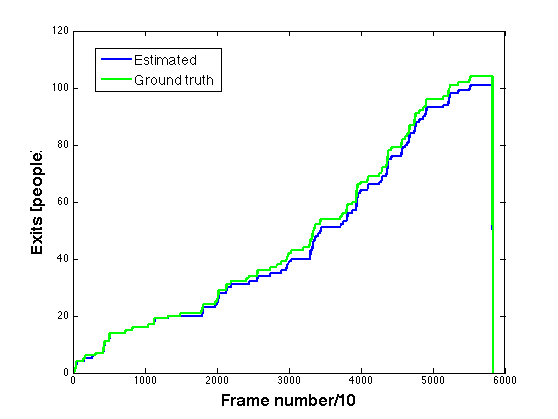
\includegraphics[width=.8\linewidth]{images/ExitsTest.png}
  \caption{Measured exits and ground truth}
  \label{fig:sub1}
\end{subfigure}%
\begin{subfigure}{.5\textwidth}
  \centering
  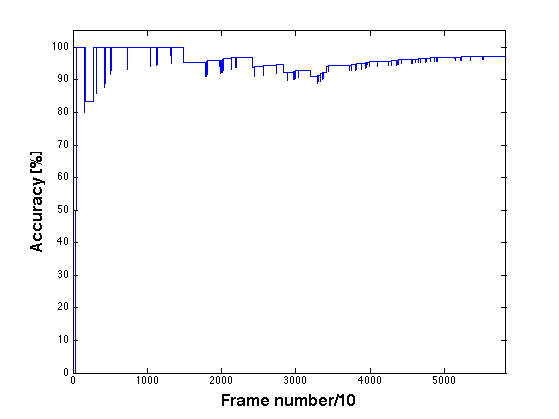
\includegraphics[width=.8\linewidth]{images/AccExitsTest.png}
  \caption{Accuracy}
  \label{fig:sub2}
\end{subfigure}
\caption[Entries training]{\textit{Training data. Plot of measured exits, ground truth and accuracy}}
\label{fig:Exits Training data}
\end{figure}


\begin{figure}[H]
\centering
\begin{subfigure}{.5\textwidth}
  \centering
  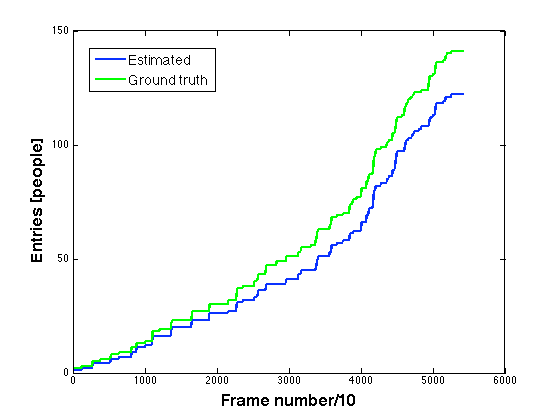
\includegraphics[width=.8\linewidth]{images/EntriesEval.png}
  \caption{Measured entries and ground truth}
  \label{fig:sub1}
\end{subfigure}%
\begin{subfigure}{.5\textwidth}
  \centering
  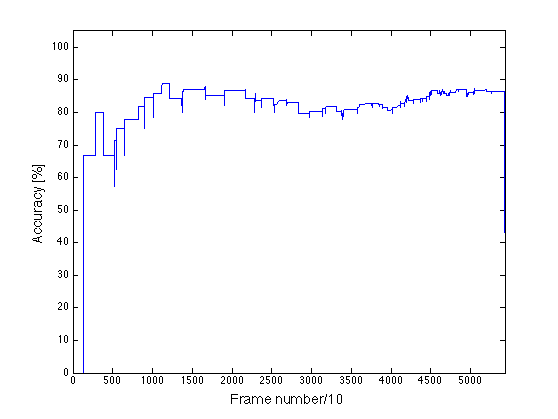
\includegraphics[width=.8\linewidth]{images/AccEntriesEval.png}
  \caption{Accuracy}
  \label{fig:sub2}
\end{subfigure}
\caption[Entries evaluation]{\textit{Evaluation data 1. Plot of measured entries, ground truth and accuracy}}
\label{fig:Entries evaluation}
\end{figure}

\begin{figure}[H]
\centering
\begin{subfigure}{.5\textwidth}
  \centering
  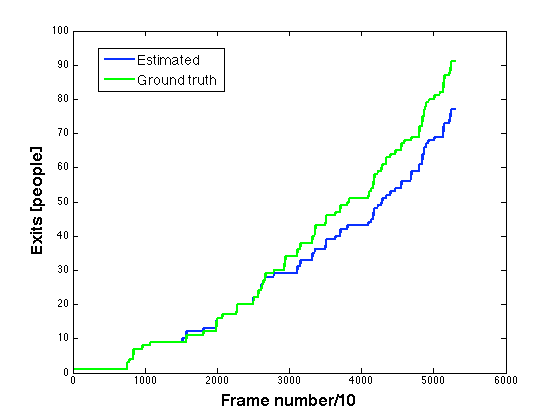
\includegraphics[width=.8\linewidth]{images/ExitsEval.png}
  \caption{Measured exits and ground truth}
  \label{fig:sub1}
\end{subfigure}%
\begin{subfigure}{.5\textwidth}
  \centering
  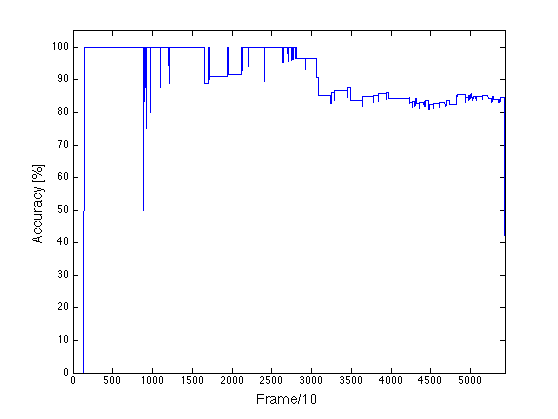
\includegraphics[width=.8\linewidth]{images/AccExitsEval.png}
  \caption{Accuracy}
  \label{fig:sub2}
\end{subfigure}
\caption[Entries evaluation]{\textit{Evaluation data 1. Plot of measured exits, ground truth and accuracy}}
\label{fig:Exits evaluation}
\end{figure}

\subsection{Discussion}
The performance of the training data set is very good. This is a sequence of 30 minutes, where only the first 5  was used in development. Evaluation data 1 performed worse, but that can be explained. The camera of this sequence was palced badly and didn't cover the entry area completely. 


